Figure~\ref{fig:4:fw} in Chapter~\ref{chap:cc.fw} shows the structure of the
congestion control framework described in this thesis. The framework
categorizes \emph{in-path} sources and \emph{in-band} signaling for
implementing congestion control (corresponds to \emph{Block A} in
Figure~\ref{fig:4:fw}), which are discussed in this chapter. This chapter is
based on our work on congestion control for interactive multimedia
applications, which is documented in \citepub{c:3grc}, \citepub{c:hetrc},
\citepub{c:eval}, \cite{rfc7097},
\cite{draft.xr.bytes.discarded}, \cite{singh:2010.thesis} and
\cite{Singh:control.loops.api}.

In \citepub{c:3grc}, we propose a new congestion control algorithm for the
mobile (e.g., 3G) environment, to be deployed in the IP Multimedia System
(IMS). The main distinction between mobile (e.g., 3G, LTE) and other wireless
environments (e.g., 802.11x) is that the media streams are transmitted using
the \emph{unacknowledged mode}; the packets corrupted due to bit-errors (e.g.,
wireless interference) are not re-transmitted. Hence, the packets incur low
delay, compared to Wireless LAN where corrupted packets are retransmitted by
the link layer. We propose a sender-driven and a receiver-driven congestion
control, and evaluate the performance of the proposed congestion control
algorithm in a simulated environment (in ns-2) using real-world 3G
traces~\cite{s4.eval.bitrate, 3gppSim}. In \citepub{c:hetrc}, we extend the
approach in \citepub{c:3grc} for deployment on the Internet and show that the
congestion control scheme is deployable there as well. In \cite{rfc7097} and
\cite{draft.xr.bytes.discarded}, we propose RTCP XR block extensions that
indicate the number of bytes discarded and run-length encoding of discarded
packets, respectively. These packets are discarded by the receiver because
they arrived too early or too late to be played out by the receiver. This
information is used as a congestion cue by the sender.

% \cite{Singh:control.loops.api} discusses the application and API requirements
% for interactive multimedia congestion control. It describes the two control
% loops: a) between the receiver and the sender, and b) between the media
% encoder and the sending agent. In the first loop, the receiver notifies the
% sender about the current network characteristics. In the second loop, the
% sending agent requests a new media bit rate, and the encoder tries at best to
% meet it, sometimes under-shooting or over-shooting the requested rate.

Lastly, in \citepub{c:eval} we evaluate the performance of a congestion
control algorithm proposed by Google for WebRTC. We evaluate the performance
in diverse scenarios measuring scalability (\emph{how quickly is the
congestion control able to utilize the available capacity}), self-fairness and
competing against bursty cross-traffic. We evaluate the performance of
web browsers implementing the congestion control algorithm in our testbed that
emulates the diverse scenarios.

\section{Schemes of Congestion Control}

The congestion control algorithm can be implemented at the sender, at the
receiver, or the sender and receiver can operate co-operatively. The
\emph{sender-driven} scheme requires that the receiver measures the current
network condition and signals the observed congestion cues to the sender, which
calculates the sender's estimate and uses it as the new sending rate. In the
\emph{receiver-driven} scheme, the receiver calculates the new sending rate
(receiver's estimate) based on the observed congestion cues, and signals the
new rate to the sender, which, on receiving the new rate, adapts the media bit
rate to the received value. The \emph{co-operative} scheme is an extension to the
\emph{sender-driven} scheme. In this case, the receiver calculates the
receiver's estimated rate and signals it along with the observed congestion
cues; the sender at its end calculates its own estimate based on the
congestion cues and chooses a new sending rate, typically a value in between the
sender's estimate and the receiver's estimate. Figure~\ref{fig:cc:scheme}
shows the interaction of the sender and receiver for each scheme. The figure
merely shows the media flow in one direction; however, it should be noted that
the media in the simulation and the emulated testbed actually flow in both
directions unless explicitly mentioned. This is mainly done for the
convenience of representation and followed throughout the remainder of the
thesis.

\subsection{Sender-driven Congestion Control Schemes}

\begin{figure}[!t]
  \centerline{
    \subfloat[Sender-driven Scheme]{
      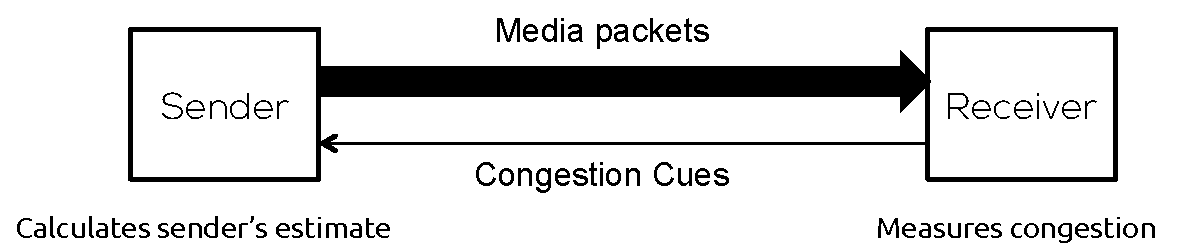
\includegraphics[width=0.9\textwidth]
      {chap5-fig-cc-scheme-s}
    }
  }
  \centerline{
    \subfloat[Receiver-driven Scheme]{
      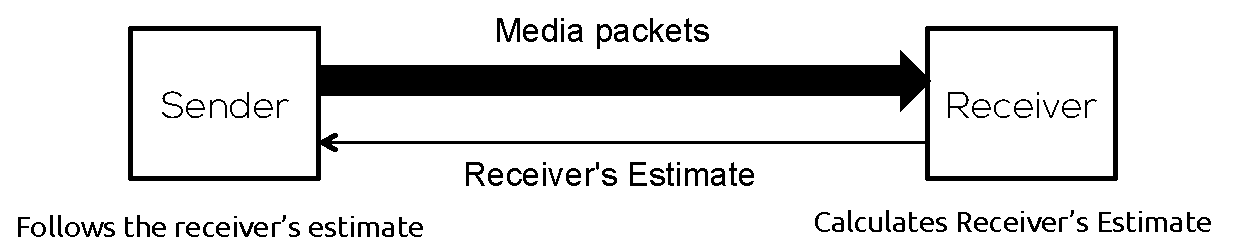
\includegraphics[width=0.9\textwidth]
      {chap5-fig-cc-scheme-r}
    }
  }
  \centerline{
    \subfloat[Co-operative Scheme]{
      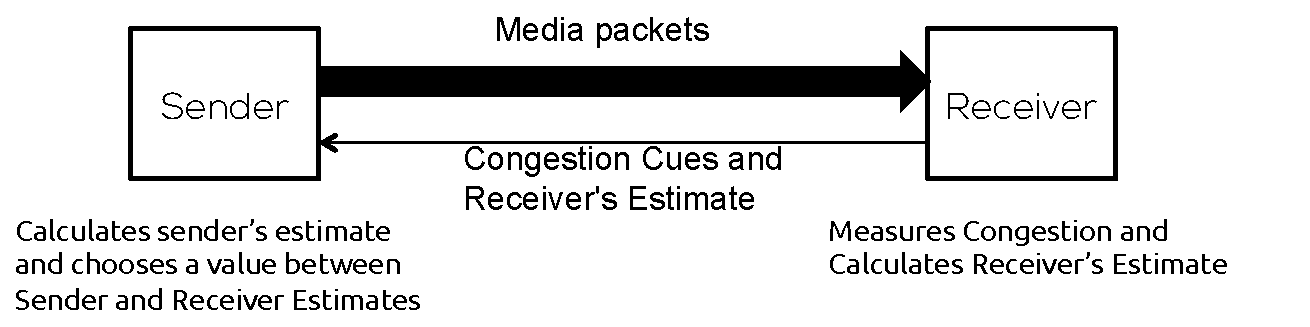
\includegraphics[width=0.9\textwidth]
      {chap5-fig-cc-scheme-c}
    }
  }
  \caption{Congestion control schemes: a) sender-driven, b) receiver-driven
and c) co-operative.}
  \label{fig:cc:scheme}
\end{figure}

TCP Friendly Rate Control (TFRC) is an equation-based congestion control
algorithm implemented at the sender~\cite{tfrc_347397} and is also implemented
as a profile~\cite{rfc4342} in the Datagram Congestion Control Protocol
(DCCP)~\cite{rfc4340}. TFRC uses the average packet size, round trip time
($RTT$), and loss ratio ($p$)~\cite{rfc3448} to calculate the new sending rate.
Formally, the sending rate in TFRC is calculated as follows:

\begin{align*}
 TFRC = &\; \frac{8 \times avg\_packet\_size}
{R \times \sqrt[]{\frac{2 \times b \times p}{3}} + t_{RTO} \times 
\left( 3 \times \sqrt[]{\frac{3 \times b \times p}{8}}\right) \times p \times
\left( 1+32 \times p^2 \right)}\\
where,\; b = &\; 1\\
t_{RTO} = &\; 4 \times R
\end{align*}

TFRC cannot directly be applied to RTP because TFRC requires per-packet
feedback, and in RTP, the RTCP feedback is not necessarily sent that
often~\cite{draft.rmcat.feedback}. Therefore, \cite{draft.rtp.tfrc} maps the
TFRC timing rules defined in~\cite{rfc4828, rfc5348} to that of the RTP/RTCP
feedback loop. It also proposes extensions to the timing rules in the
AVPF-profile~\cite{rfc4585} for very short RTTs ($<20ms$).
\cite{Gharai06:ICME} and \cite{VladBalan:2007dq} show that TFRC is stable on
paths with longer RTTs than those with smaller RTTs, but it too exhibits
saw-tooth behavior~\cite{saurin:2006:thesis}. Any algorithm that consistently
produces a sawtooth media rate is not well suited for real-time communication
because it generates a poor user-experience~\cite{Gharai:2002wt,
Zink03subjectiveimpression}.

Other sender-driven congestion control algorithms that we explored include the
Rate Adaption Protocol (RAP)~\cite{rap:752152} that uses a windowed approach which 
exhibits a sawtooth-type of behaviour. Zhu~\textit{et
al.}~\cite{rmcat-nada} use Pre-Congestion Notification (PCN), Explicit
Congestion Notification (ECN) and loss rate to get an accurate delay
estimate for implementing congestion control. In this case, they assume all
packets marked by ECN and PCN as lost. Their algorithm as specified now, 
relies on accurate measurement of one-way delay relying on clock synchronization.
Instead of just relying on RTT and loss for congestion control, 
Garudadri~\textit{et al.}~\cite{4397059} also use the
receiver playout buffer to detect the link utilization, i.e., the variation in the 
receiver playout buffer occupancy indicates an increase or decrease in congestion.
O'Hanlon~\textit{et al.}~\cite{rmcat-dflow} propose using a delay-based
estimate when competing with similar traffic and, using a windowed-approach
when competing with TCP-type cross traffic, they switch modes by applying a
threshold on the observed end-to-end delay. The idea is similar to the one
discussed in~\cite{budzisz2011fair}.




\subsection{Receiver-driven Congestion Control Schemes}

In receiver-driven congestion control, the receiver estimates the rate and
notifies the sender about the new sending rate. Temporary Maximum Media 
Bit-rate Request (TMMBR) is defined as a codec control message in \cite{rfc5104}.
It is generated by the receiver in a point-to-point video call. The receiver
calculates the new estimate (available capacity) based on the average 
inter-arrival time of RTP packets (\emph{video frames}). When the inter-arrival time
of the video frames increases beyond the expected arrival time in an observed
period, the receiver senses \emph{over utilization}. When the frames arrive early, the
receiver senses \emph{under utilization}. The receiver ignores the congestion event 
if it occur on short timescales and when receiving I-frames. 
The I-frames are large frames because they are spatially compressed and
are not temporally correlated to previous frames. Hence, these I-frames are
expected to cause queuing delay. The receiver, on detecting link over
or under utilization, modifies the \emph{receiver's capacity estimate}. 
The receiver sends the TMMBR message to the sender
indicating the maximum sending rate. Currently, interactive multimedia sessions
in 3GPP~\cite{3gpp.26.114} use TMMBR messages to notify the sender of the
expected sending rate. In WebRTC~\cite{jennings:2013:webrtc}, TMMBR is
expected to be used initially, before RTP congestion control is standardized
by the IETF~\cite{rtp-usage}. The expectation is that different WebRTC clients
may develop proprietary receiver-driven algorithms and use TMMBR as the
standardized mechanism to communicate the capacity estimate to the sender,
which will blindly follow it.


\subsection{Co-operative Congestion Control Schemes}
\label{cc:co-op}

The Next Application Data Unit (NADU)~\cite{nadu.1070341,nadu.1530486} is designed
for rate adaptation for video streaming in 3GPP~\cite{3gpp.26.234}. A NADU
receiver measures the playout delay (as a measure of buffer occupancy in time)
and signals it to the sender along with the next sequence number to be played
out. Conversational NADU (C-NADU) is an extension of NADU for congestion
control for interactive multimedia and is described in \citepub{c:3grc} and
\citepub{c:hetrc}. In C-NADU, the receiver also calculates the
\emph{receiver's capacity estimate} by measuring the frame inter-arrival time
and signals that along with the NADU report. If the video frame arrives at the
expected time, the receiver assumes no ongoing congestion, and if it arrives
later than the expected time, the frame is considered late and the receiver
diagnoses congestion. If the frame is delayed and misses its playout time, it
is discarded and in this case the receiver estimates congestion. Based on the
above cases, the receiver estimates the current capacity and signals it to the
sender. At the sender, the C-NADU controller calculates the TCP-friendly rate,
measures the variation in RTT ($75$ and $90$ percentile values) and calculates
the fraction of video frames that missed their playout deadline. Based on
these congestion cues and the receiver estimate, the sender chooses a new
sending rate.


Receiver-side Real-Time Congestion Control (RRTCC) is described in
\cite{draft.rrtcc} and is proposed as one of the solution candidates for
WebRTC by Google. Like C-NADU, RRTCC also has a receiver- and sender-side
component. The receiver-side measures the under or over utilization by
monitoring the timestamp jitter of the incoming frames. The arrival times are
modeled as a white Gaussian process. When the mean is 0 there is no
congestion; the mean is expected to increase when there is ongoing congestion
and expected to decrease when the congestion abates. Based on this
expectation, the receiver calculates the capacity estimate and signals it to
the sender. The sender calculates its estimate based on TFRC, and finally,
chooses the new sending rate as a value between the TFRC rate calculated by
the sender and the receiver's estimate. Full details of the algorithm proposed by
Google are documented in an Internet-Draft~\cite{draft.rrtcc}.



\begin{figure}[!t]
  \centerline{
    \subfloat[TFRC]{
      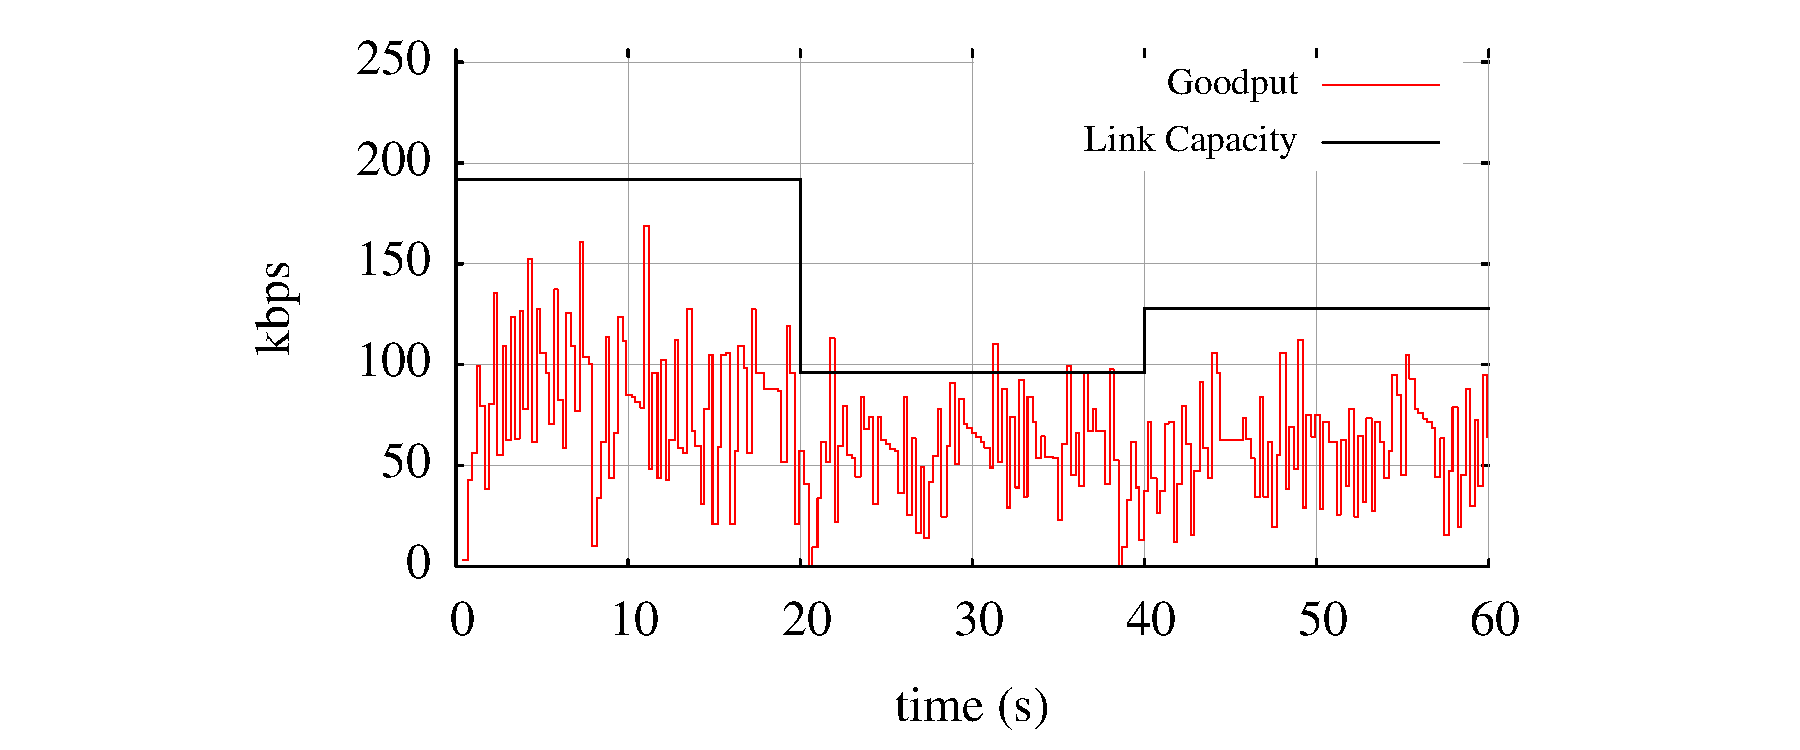
\includegraphics[width=0.5\textwidth, clip=true, trim=3cm 0 4.5cm 0]
      {chap5_graph_sl_tfrc}
    }
    \subfloat[TFRC]{
      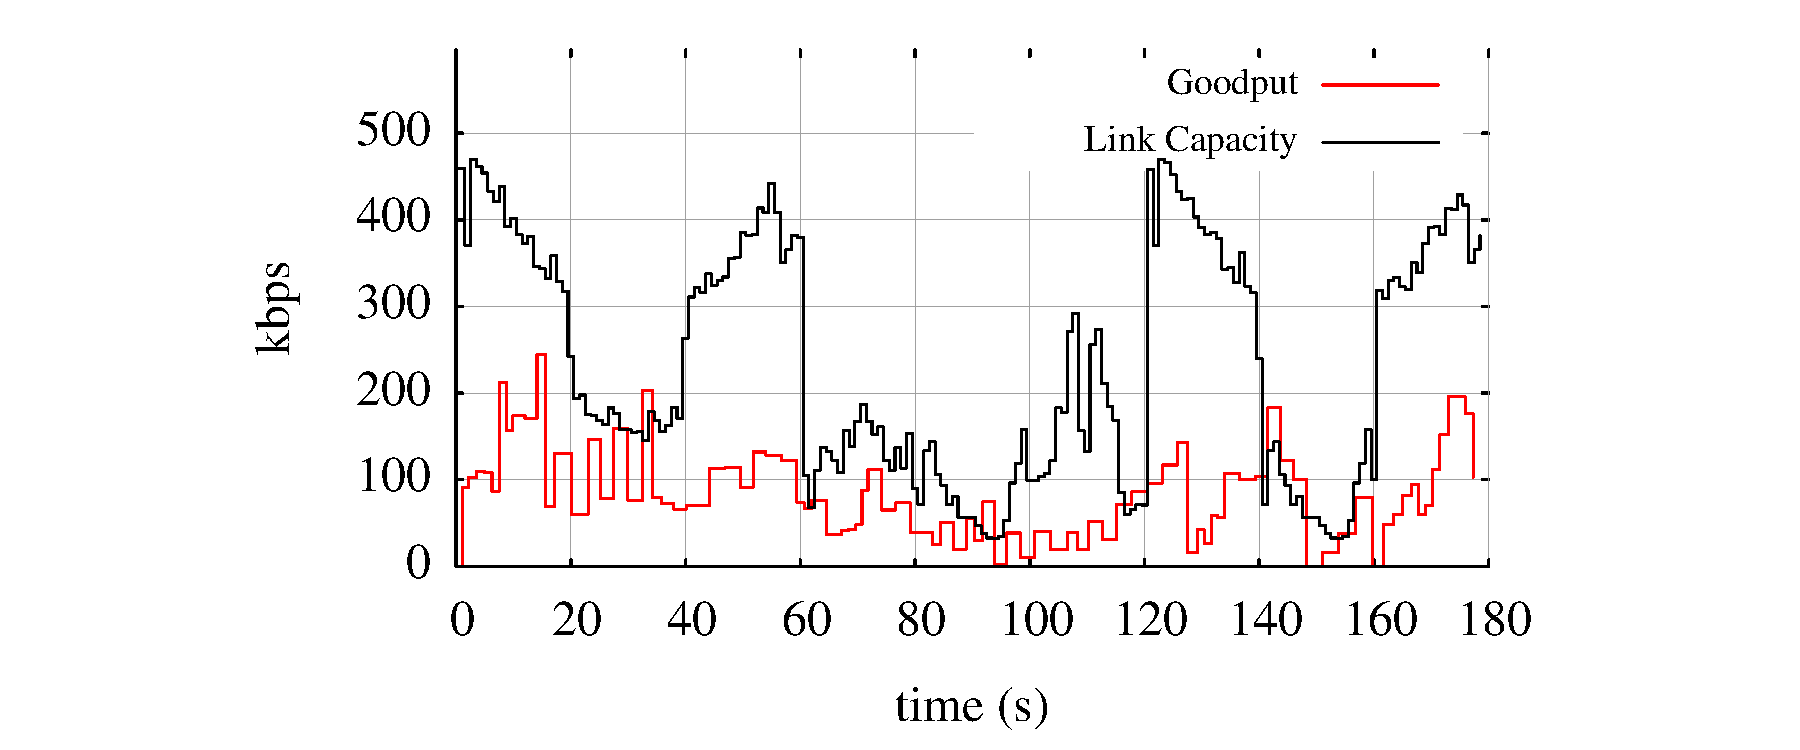
\includegraphics[width=0.5\textwidth, clip=true, trim=3cm 0 4.5cm 0]
      {chap5_graph_3g_tfrc_1}
    }
  }
  \centerline{
    \subfloat[TMMBR]{
      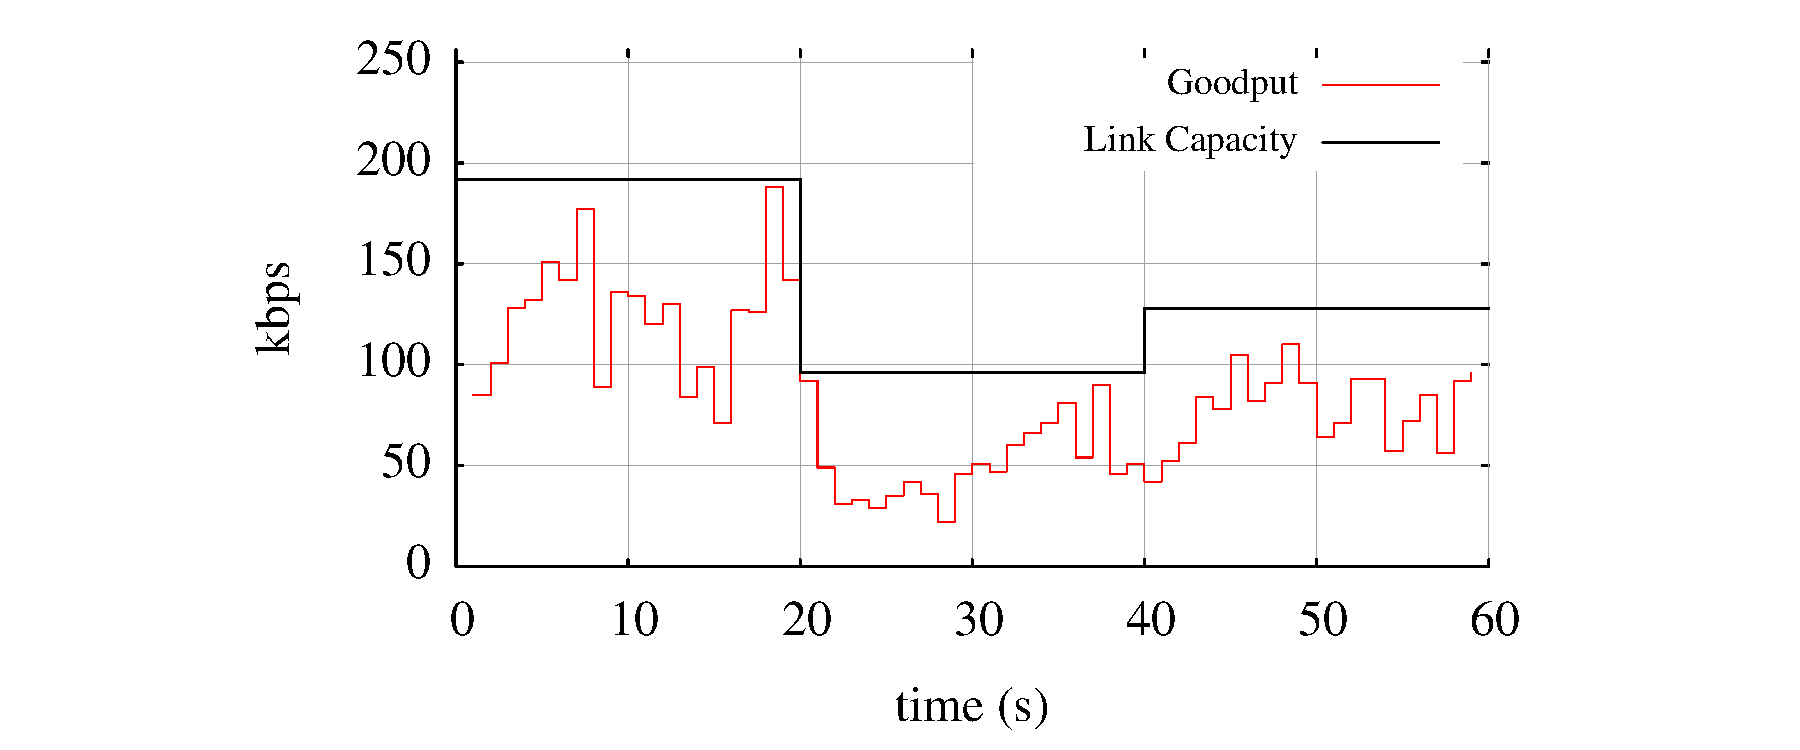
\includegraphics[width=0.5\textwidth, clip=true, trim=3cm 0 4.5cm 0]
      {chap5_graph_sl_tmmbr}
    }
    \subfloat[TMMBR]{
      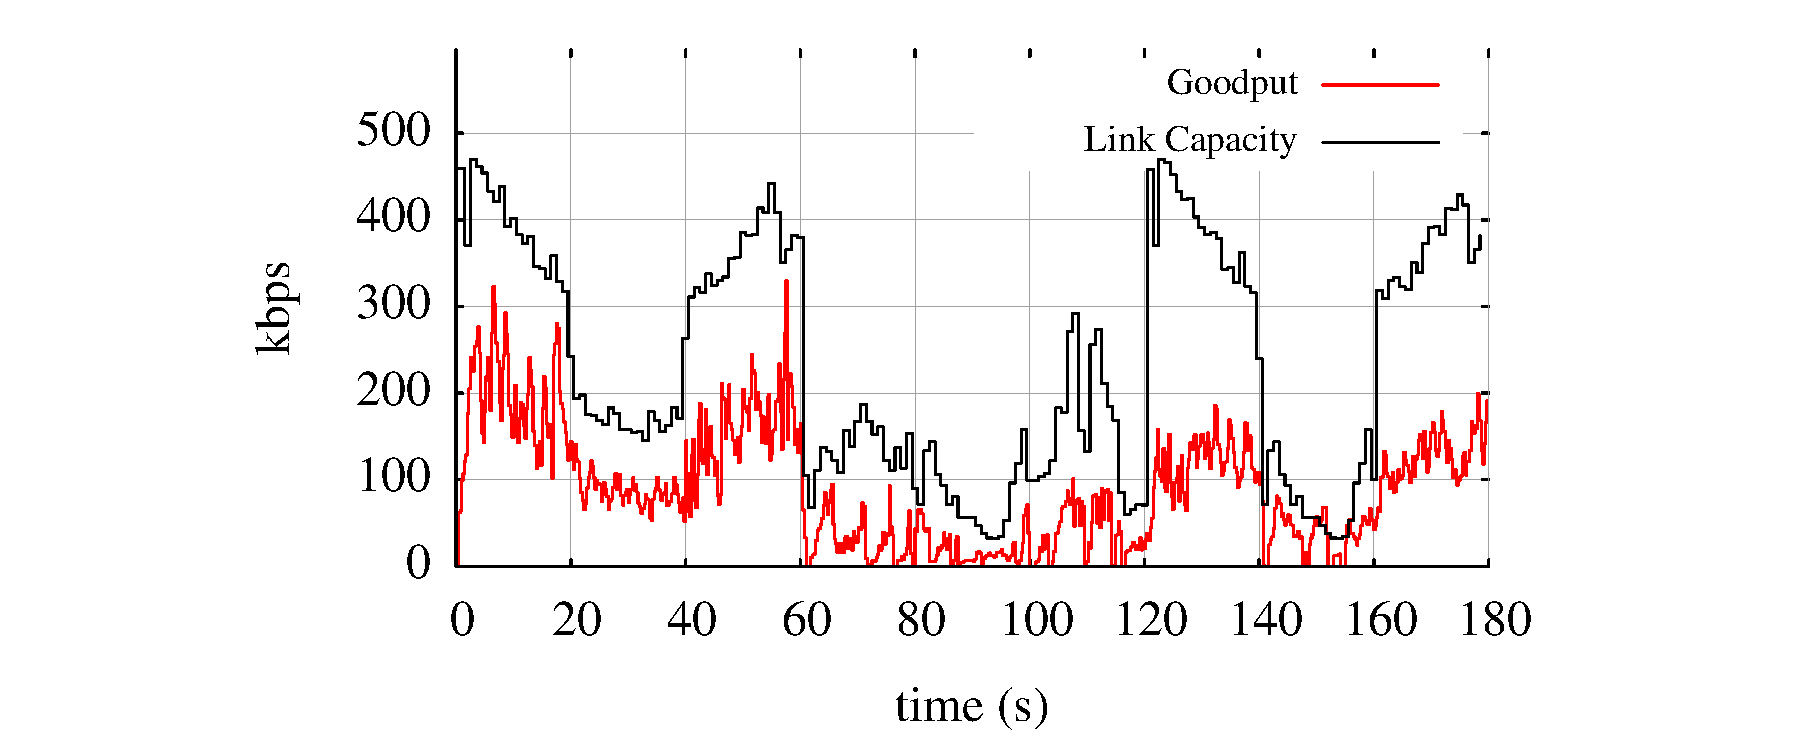
\includegraphics[width=0.5\textwidth, clip=true, trim=3cm 0 4.5cm 0]
      {chap5_graph_3g_tmmbr_u}
    }
  }
  \centerline{
    \subfloat[C-NADU]{
      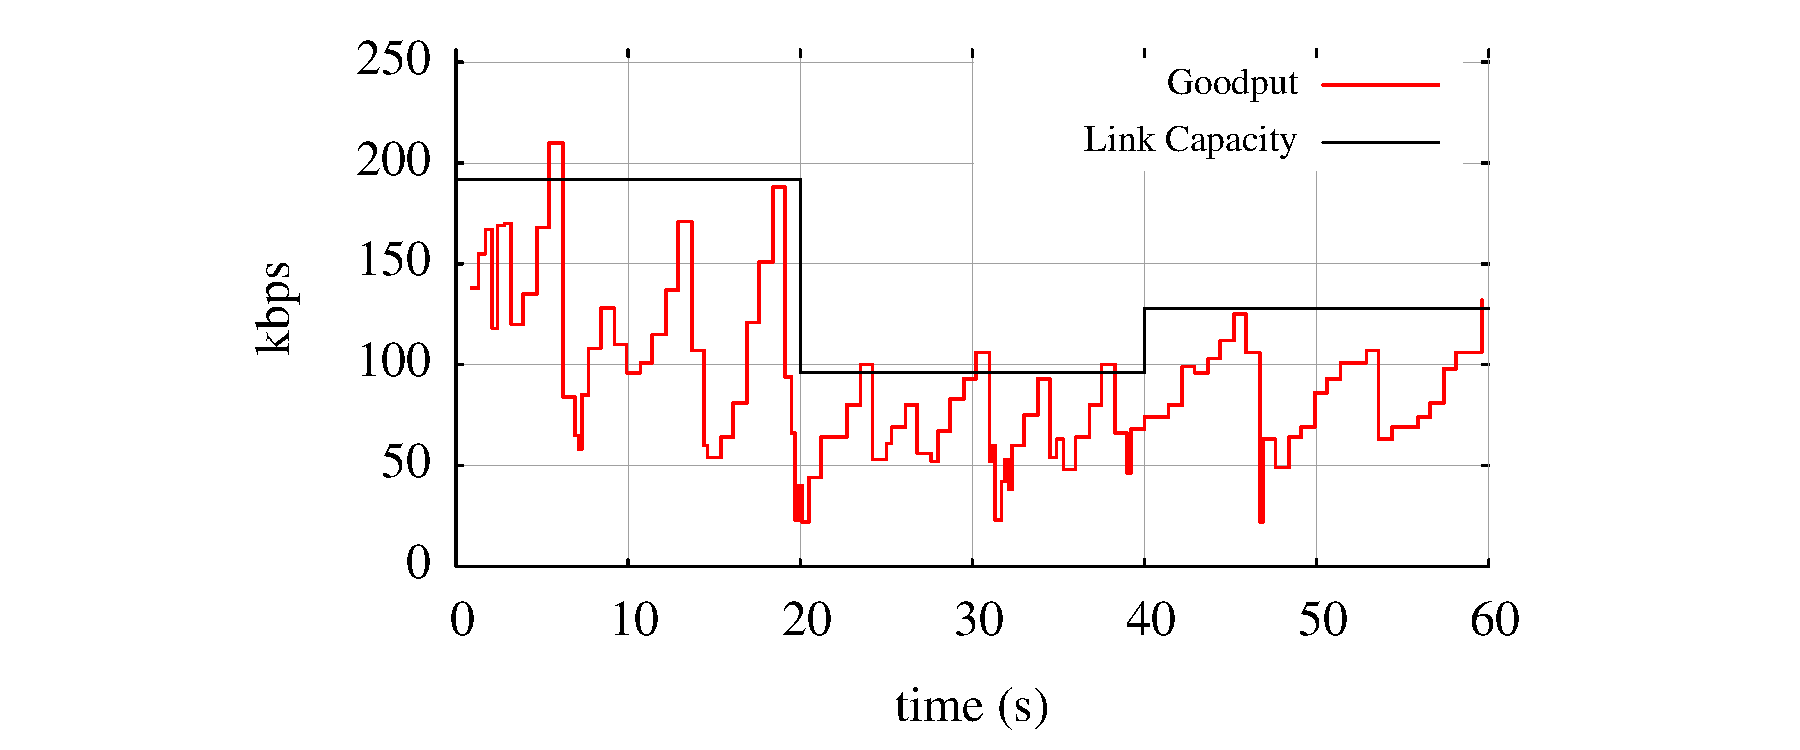
\includegraphics[width=0.5\textwidth, clip=true, trim=3cm 0 4.5cm 0]
      {chap5_graph_sl_cnadu}
    }
    \subfloat[C-NADU]{
      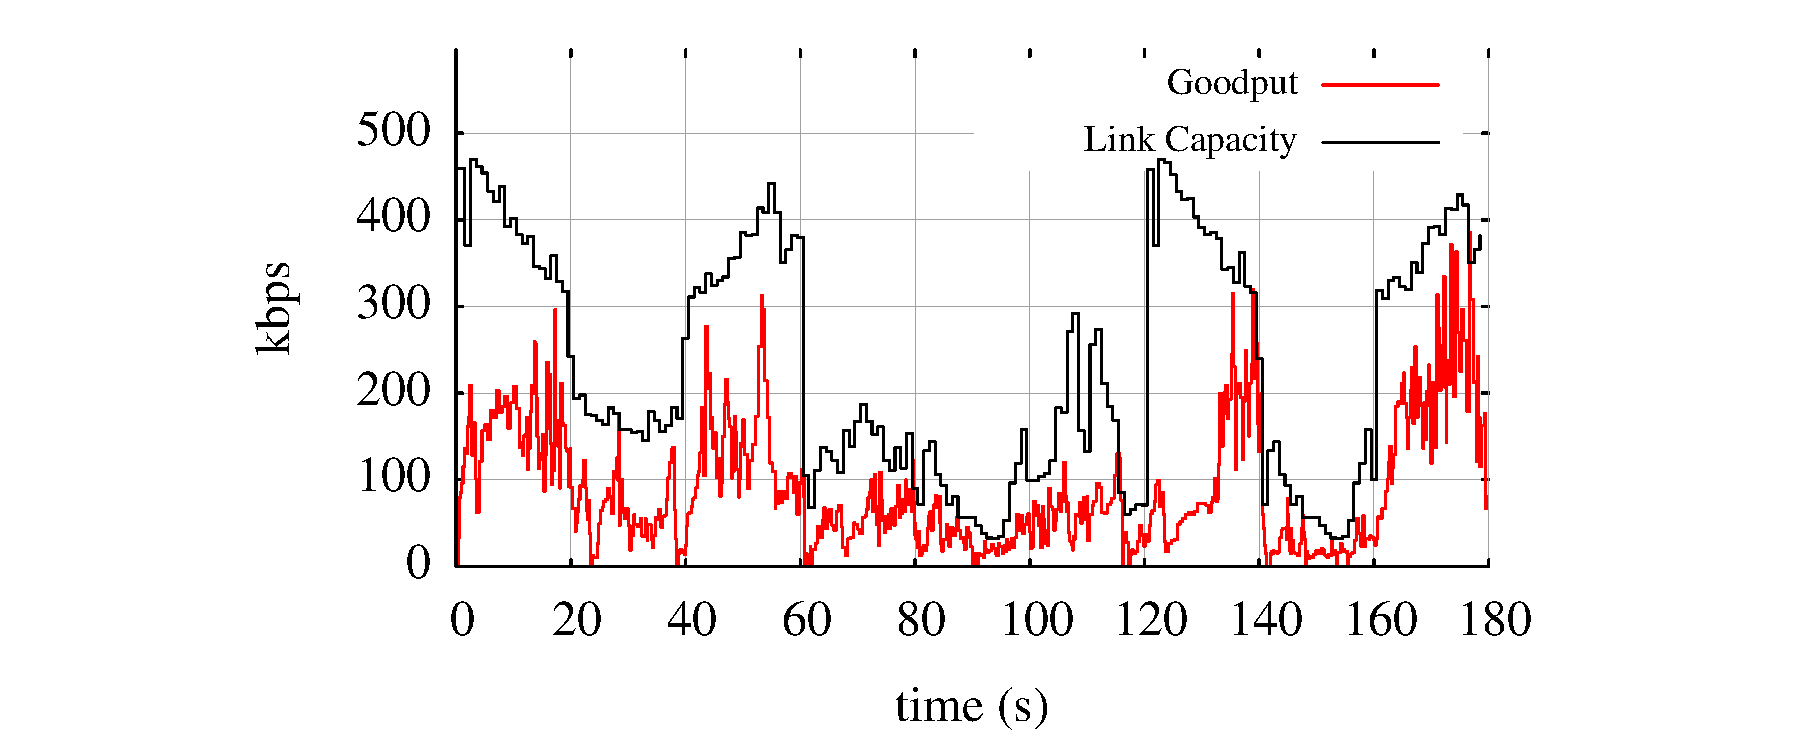
\includegraphics[width=0.5\textwidth, clip=true, trim=3cm 0 4.5cm 0]
      {chap5_graph_3g_cnadu}
    }
  }
  \caption{TPerformance of TFRC, TMMBR and C-NADU in a slow
  time-varying link (a, c, e) and 3G network (b, d, f).}
  \label{fig:3grc}
\end{figure}


\begin{table}[!t]
\centering{
\begin{tabular}{cccc}
\hline
 & $Goodput_{avg}$ & PLR & $PSNR_{avg}$\\
 & (Kbps)  &(\%) & (dB)\\
\hline
TFRC & 84.1 & 6.9\,\%& 29.3 \\ %
TMMBR & 89.8 & 3.7\,\% & 30.5 \\ %
%NADU & 106 & 93 & 29.9& 6.3\%\\%
C-NADU & 92 & 2.2\,\% & 31.9 \\%
\hline
\end{tabular}
}
\caption{Comparing TFRC, TMMBR, C-NADU for calls over mobile nodes (180\,\emph{s}
simulations using 3G traces).}
\label{table:3grc}
\end{table}

\section{Performance Analysis of TFRC, TMMBR, C-NADU, and RRTCC}

This section briefly discusses the performance of each congestion control
algorithm. The detailed analysis can be found in the respective papers.

Our results in \citepub{c:3grc} show that TFRC produces a sawtooth sending
rate, similar to the performance in~\cite{saurin:2006:thesis}. When the media
stream is the only flow on the end-to-end path, we also observe that the average
bandwidth utilization (ABU) is between 30-40\,\%, i.e., TFRC under utilizes the
link and the loss ratio is about 6\,\%, which results in a lower media quality
(approximated by measuring PSNR) compared with the other two schemes (see
Table~\ref{table:3grc}). TMMBR-based congestion control utilizes the link
better than TFRC (ABU between 50-70\,\%) and produces a lower loss ratio
($\approx$3\,\%). Lastly, C-NADU has comparable bandwidth utilization
(ABU=55-60\,\%) and loss ratio ($\approx$2\,\%) to TMMBR.
Figure~\ref{fig:3grc} shows the performance of TFRC, TMMBR and C-NADU over two
types of bottleneck links, a slow time-varying link and a 3G link.


\begin{figure}[!t]
\centerline{
%\hfill
\subfloat [Call 1 vs Call 2] {\label{fig_sim-mixed-1-1}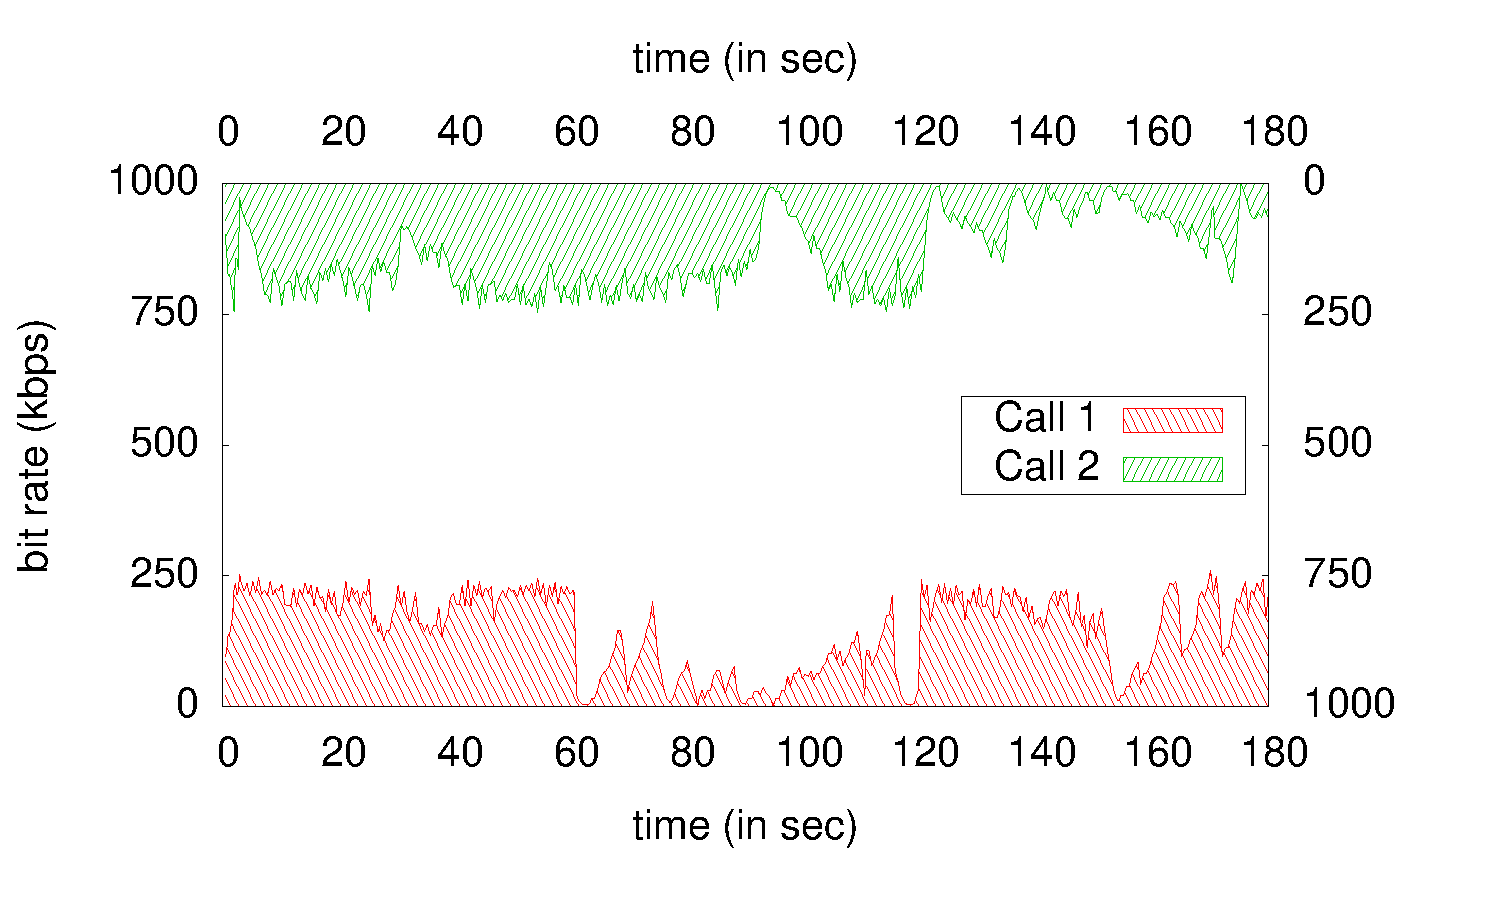
\includegraphics[width=0.5\textwidth]{chap5-graph-5rtp_uc1_12}%
}
%\hfill
\subfloat [Call 1 vs Call 3] {\label{fig_sim-mixed-1-2}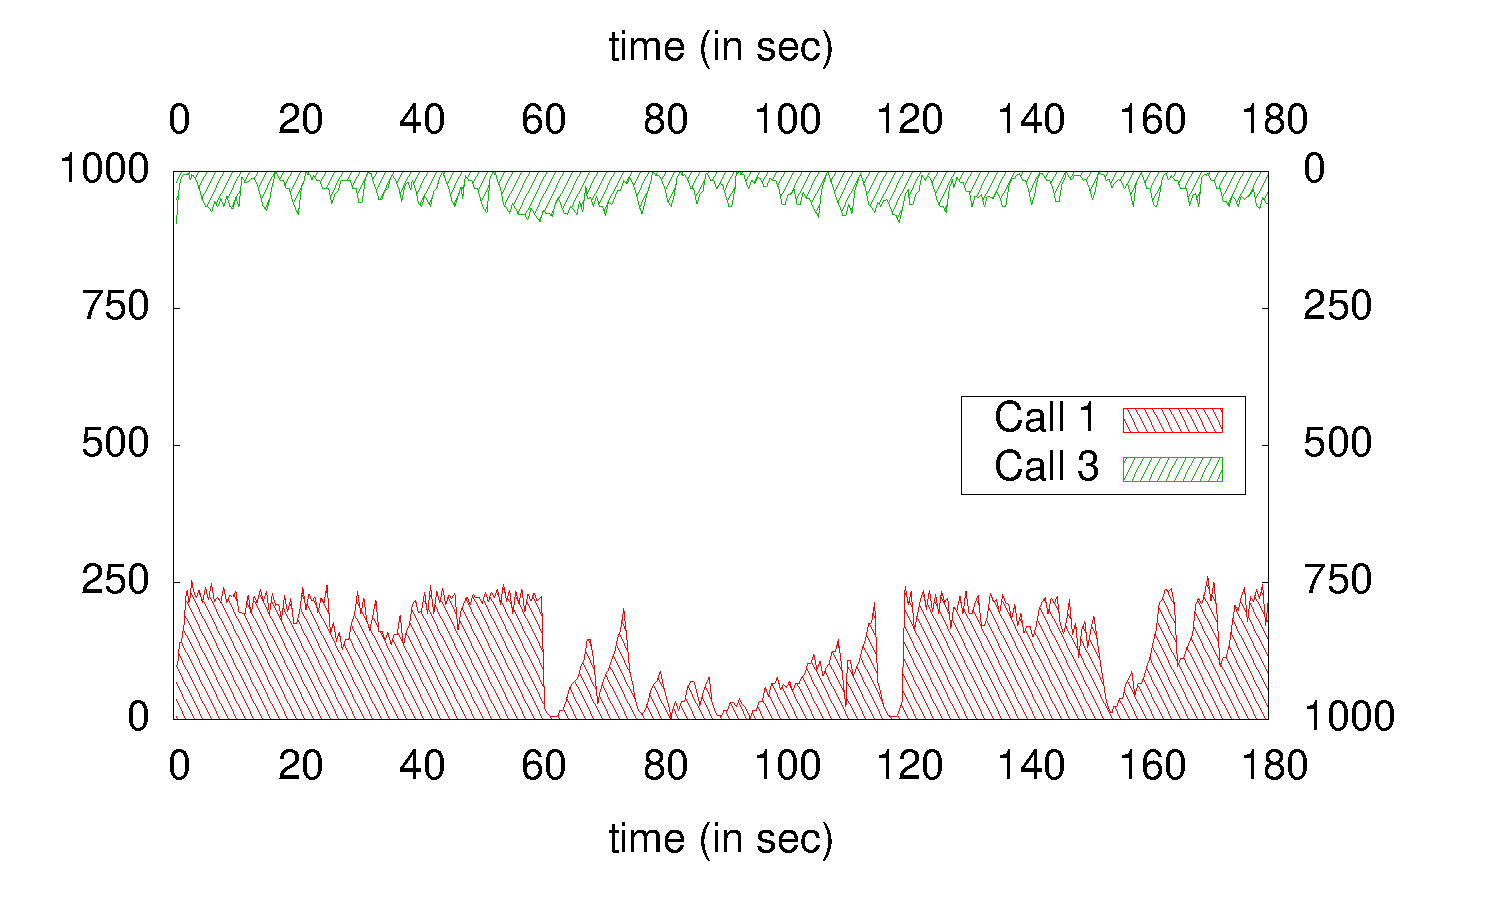
\includegraphics[width=0.5\textwidth]{chap5-graph-5rtp_uc1_13}%
}
%\hfill
}
\centerline{
%\hfill
\subfloat [Call 1 vs Call 4] {\label{fig_sim-mixed-1-3}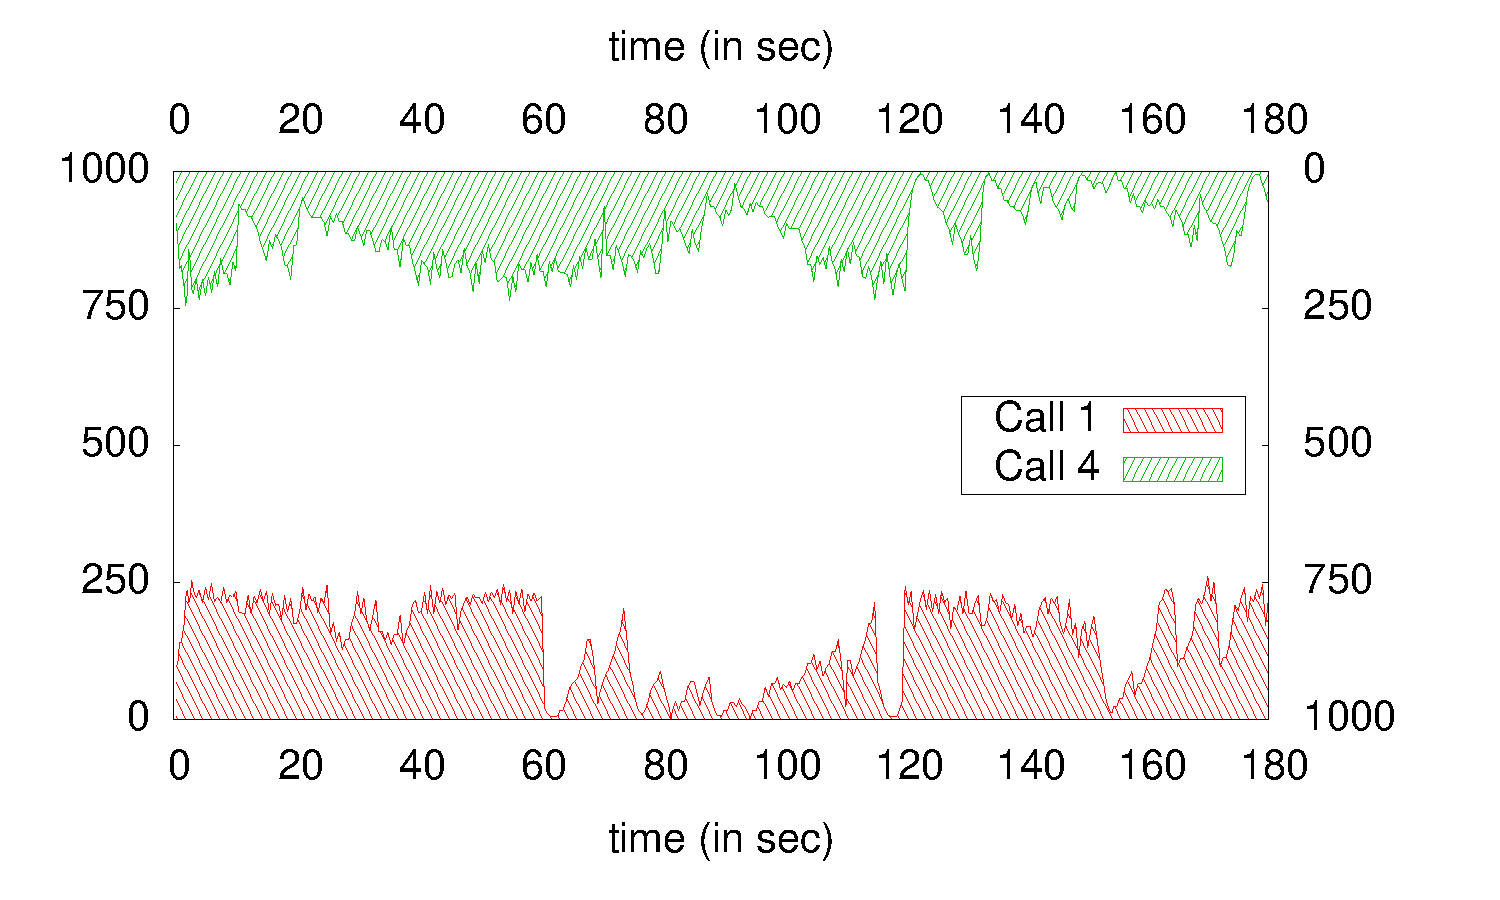
\includegraphics[width=0.5\textwidth]{chap5-graph-5rtp_uc1_14}%
}
%\hfill
\subfloat [Call 1 vs Call 5] {\label{fig_sim-mixed-1-4}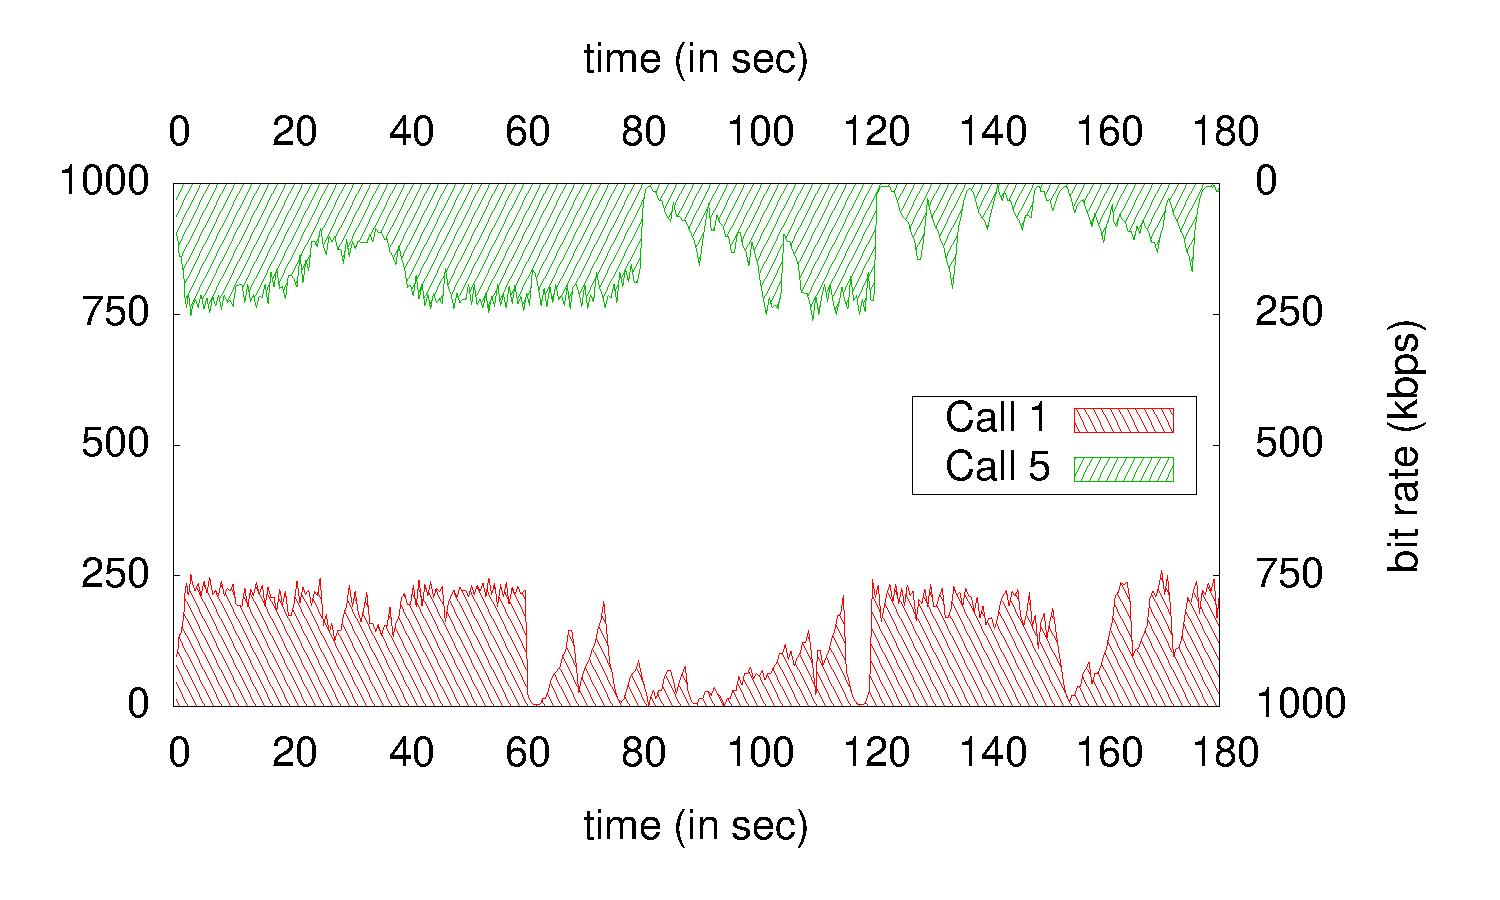
\includegraphics[width=0.5\textwidth]{chap5-graph-5rtp_uc1_15}%
}
%\hfill
}
\caption{Performance of five C-NADU calls competing for
capacity on a shared bottleneck in a heterogeneous network. Each call needs
to quickly adapt to changes in 3G link capacity and fairly share the
bottleneck link.}
\label{fig:hetrc}
\end{figure}

\begin{table}[!t]
\centering{
\scalebox{0.9}{
\begin{tabular}{cccccc}
\hline
 & 3G Capacity & $Goodput_{avg}$ & PLR & $PSNR_{avg}$ & ABU \\
 & Pattern & (Kbps) & (\%) & (dB) ($\sigma$)  & (\%) \\ 
\hline
Call 1 & Excellent-Poor-Elevator & 140.10 & 2.15\,\% & 31.4 ($0.39$) & 70.1\,\% \\ 
Call 2 & Good-Good-Poor & 133.55 & 1.61\,\% & 31.9 ($0.62$)& 66.8\,\% \\ 
Call 3 & Poor-Poor-Poor & 35.18 & 1.55\,\% & 22.2 ($1.13$)& 17.59\,\% \\ 
Call 4 & Fair-Fair-Poor & 114.96 & 2.75\,\% & 31.1 ($0.75$)& 57.5\,\% \\ 
Call 5 & Excellent-Elevator-Poor & 130.23 & 2.25\,\% & 31.3 ($0.13$)& 65.1\,\% \\ 
\hline
\end{tabular}
}}
\caption{C-NADU: Five calls in a heterogeneous network with end-to-end latency
between 60-120\,\emph{ms} and 0.5\,\% link-layer losses.}
\label{table:hetrc}
\end{table}

In \citepub{c:hetrc}, we show that C-NADU is self-fair with other C-NADU flows
in both wired and wireless environments~\cite{singh:2010.thesis}, and in
\citepub{c:fecrc} we show that it competes fairly with TCP cross-traffic, for both
the long- and short-TCP flows. Figure~\ref{fig:hetrc} show five video calls in which
each sender uses an independent 3G link into a common bottleneck to the
receivers. The 3G links are based on radio link traces and have different
capacities. Hence, at some instances of time, the 3G link is the constraint and
at other times it is the shared bottleneck link. Table~\ref{table:hetrc} shows that
four calls have comparable performance (see PSNR and goodput) and one call suffers
due to poor connectivity (the 3G link has insufficient capacity which affects
the quality).

\begin{figure}[!t]
  \centerline{
    \subfloat{
      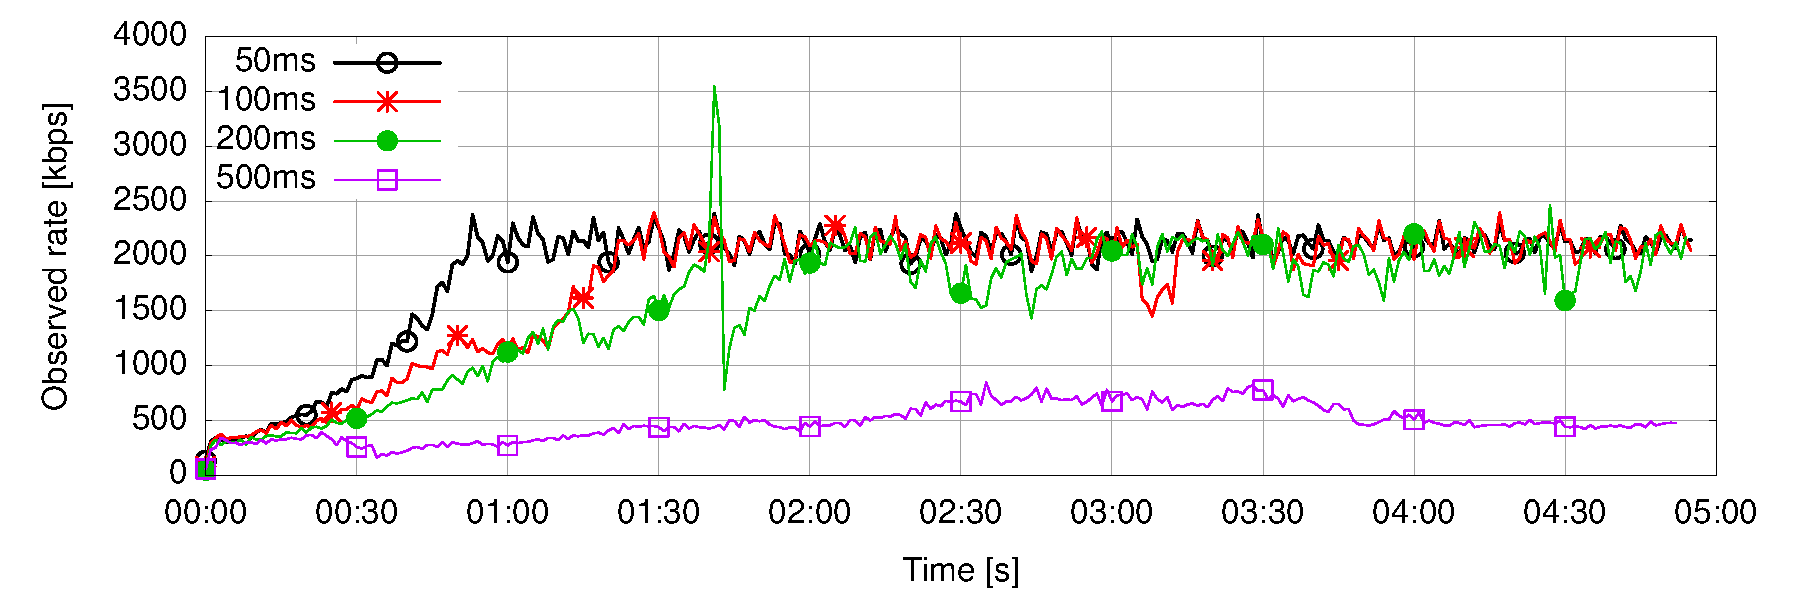
\includegraphics[width=0.8\textwidth]
      {chap5-graph-rrtcc-latency}
    }
   }
   \centerline{
    \subfloat{
      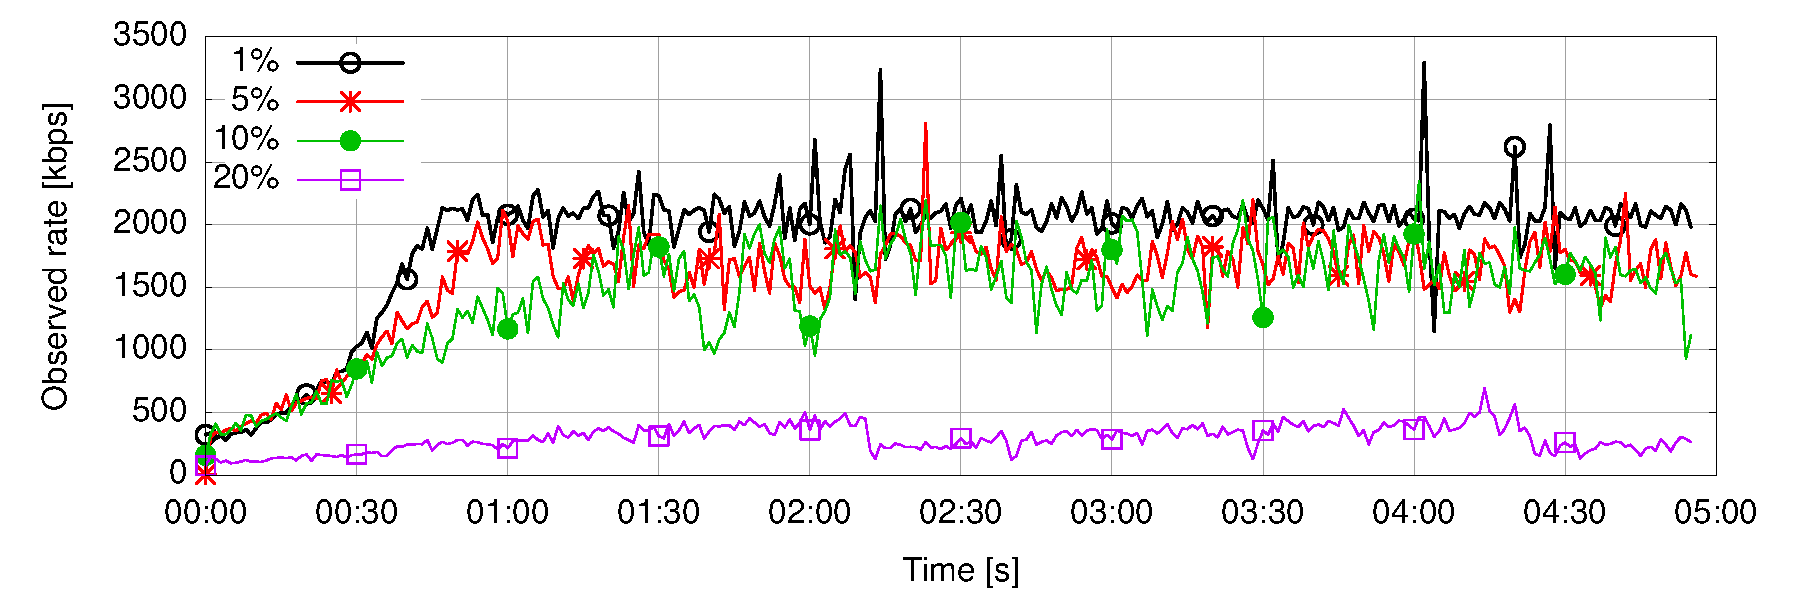
\includegraphics[width=0.8\textwidth]
      {chap5-graph-rrtcc-plr}
    }
  }
  \caption{The plots show the performance of RRTCC on a link with varying
  delay and fractional loss rate. We observe that by the sending rate
  decreases with increasing link latency or bit-error loss. }
  \label{fig:rrtcc-single}
\end{figure}

\begin{table}[!t]
\begin{center}{
  \scalebox{0.9}{
\begin{tabular}{ ccccc }
\hline
 & $Goodput_{avg}$ & Residual  & PLR\\
 & (Kbps)  & Loss (\%) & (\%)\\
\hline
 0\,\% & 1949.7 $\pm$ 233.62 & 0.011 & 0.011 \\ 
 5\,\% & 1568.74 $\pm$ 178.52 & 0.23 & 9.77 \\ 
 10\,\% & 1140.82 $\pm$ 161.92 & 0.49 & 19.02 \\ 
 20\,\% & 314.4 $\pm$ 61.98 & 2.43 & 36.01 \\ \hline
\end{tabular}
}}
\end{center}
\caption{RRTCC: Metrics for a bottleneck with different packet loss rates.}
\label{tab:rrtcc-loss}
\end{table}

In \citepub{c:eval}, we evaluate the performance of RRTCC in several
scenarios: by itself on a bottleneck link, competing with other RRTCC flows
and competing with TCP cross-traffic. Figure~\ref{fig:rrtcc-single} shows an
example plot of the performance of RRTCC. In Figure~\ref{fig:rrtcc-single}(a) when
increasing the bottleneck link latency reduces the sending rate of RRTCC.
Similarly, Figure~\ref{fig:rrtcc-single}(b) shows that when increasing the loss
rate also affects the sending rate. However, Table~\ref{tab:rrtcc-loss} shows
that even though the link has a high loss rate, the residual loss rate is low
(even when the loss was 20\,\%), mainly due to the use of NACKs, PLI and FEC.


\begin{figure}[!t]
\centerline{
  \subfloat[Start together]
    {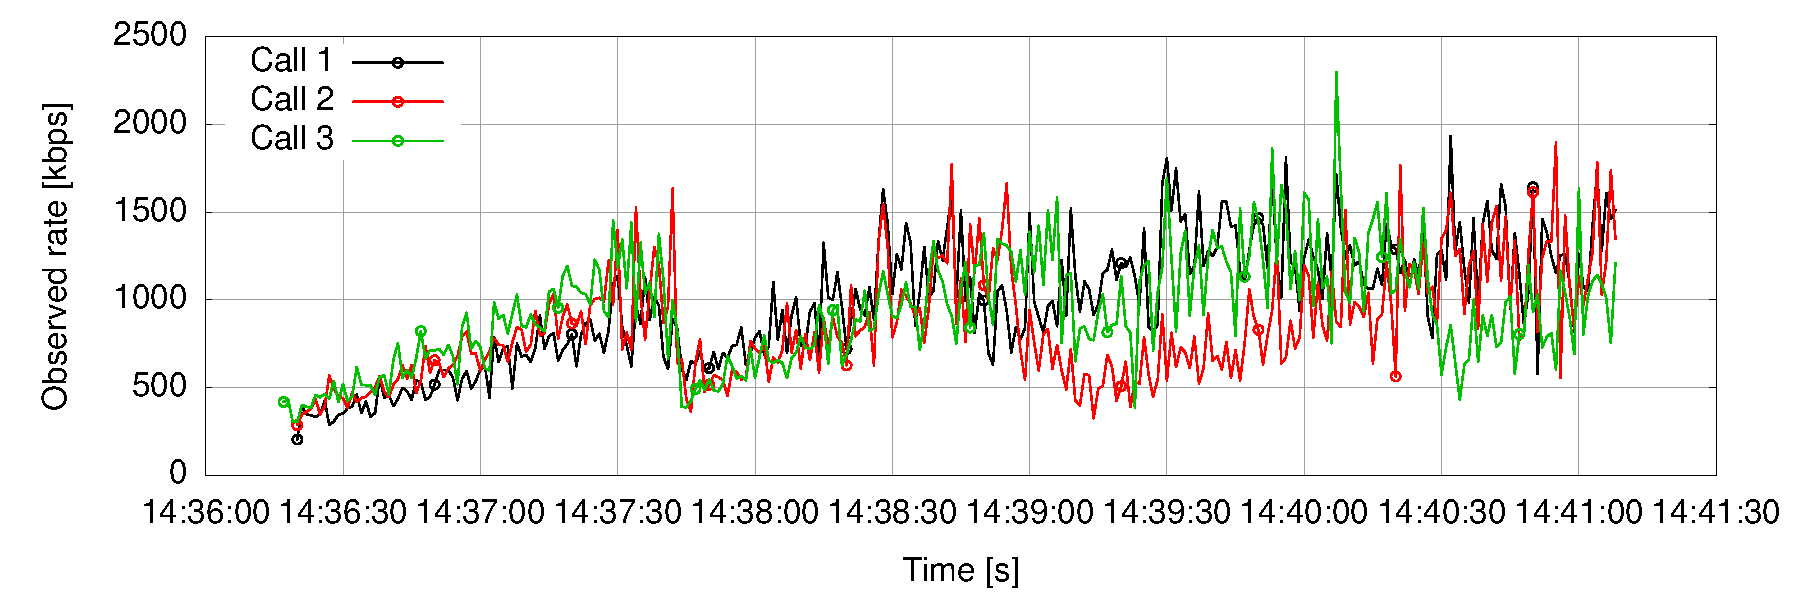
\includegraphics[width=0.8\textwidth]
    {chap5-graph-rrtcc-three-calls-sync}}
  }
  \centerline{
  \subfloat[Start 30\,\emph{s} apart]
    {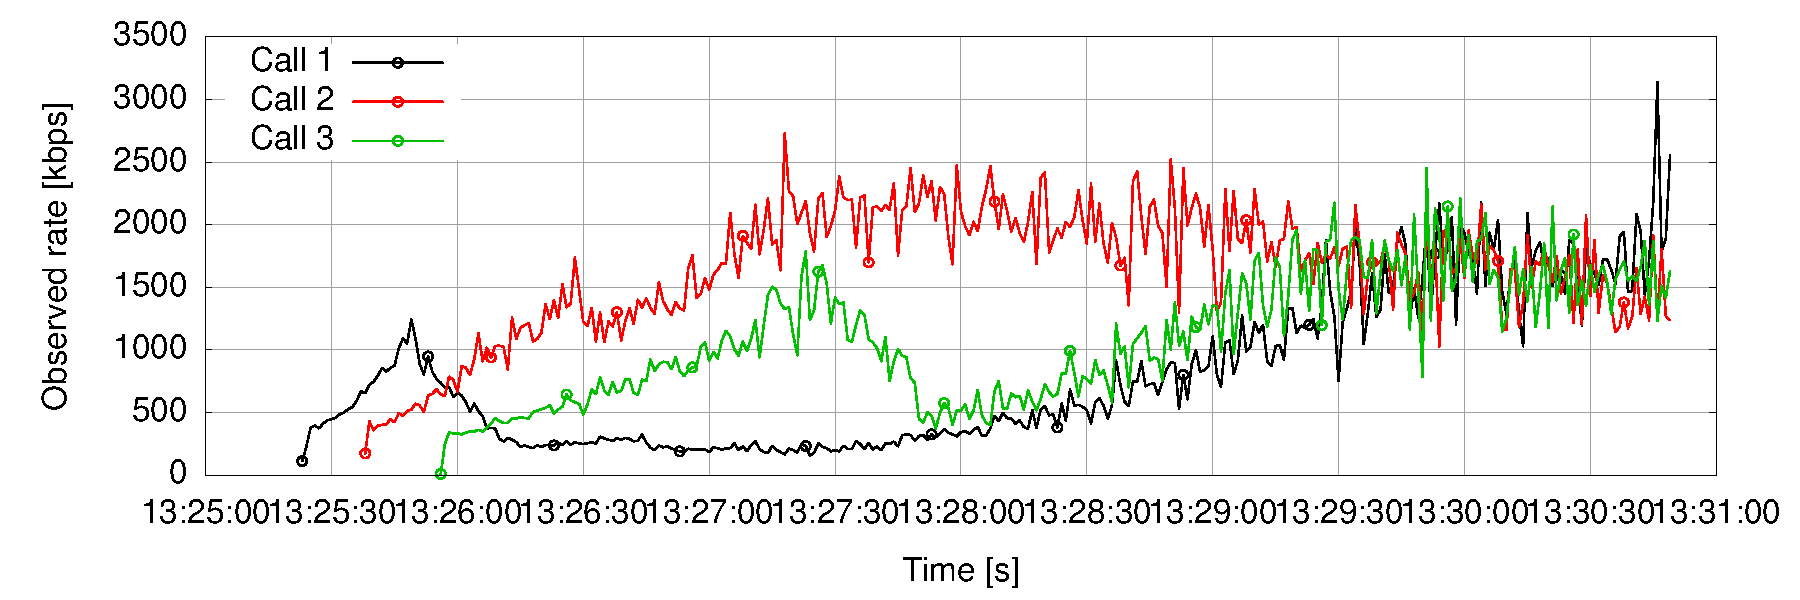
\includegraphics[width=0.8\textwidth]
    {chap5-graph-rrtcc-three-calls-async}}
  }
   \caption{The plots show the variation in receiver rate of three RRTCC
   flows, a) starting together, b) starting 30\,\emph{s} apart. The total duration of
   the call is 5 mins (300\,\emph{s}).}
\label{fig:rrtcc-self-fair}
\end{figure}

\begin{table}[!t]
\begin{center}
  \scalebox{0.9}{
\begin{tabular}{ccccc}
\hline
& $Goodput_{avg}$  & RTT & Residual & PLR\\
& (Kbps)& (ms) & Loss (\%) & (\%)\\ \hline
 3 calls &  809.07 $\pm$ 202.38 &   31.48 $\pm$ 24.93 & 0.21 & 0.23 \\  
 3 calls (time shifted) &  1154.32 $\pm$ 250.54 &   35.15 $\pm$ 27.88 & 0.08 & 0.91 \\ \hline
\end{tabular}
}
\end{center}
    \caption{RRTCC competing with similar cross-traffic on the bottleneck link.}
    \label{tab:self-fair}
\end{table}

Next, we emulate three calls sharing a common bottleneck. In this case, the
individual media rates do not reach their individual maximum rate of 2\,\emph{Mbps}.
Figure~\ref{fig:rrtcc-self-fair}(a) shows that the three calls ramp up at about the
same rate, reach a peak and drop their rate simultaneously. The sending rates
synchronize, even though the flows originate from different endpoints using
independent RTP stacks.

Lastly, instead of the three calls starting together, each call starts at 30\,\emph{s}
intervals. We observe that while the media rate per call on average is higher,
the first call has a disadvantage. In all the cases, the first media flow temporarily 
starves when a new flow appears, ramping up again after a few minutes.
Figure~\ref{fig:rrtcc-self-fair}(b) shows the instantaneous rates of each of
the calls. The first call temporarily starves when new flows appear because,
when it starts, it is the only flow on the bottleneck and does not encounter
any queues; it observes a certain RTT and uses that as the baseline. When the
second flow appears, the second flow already observes queues from the existing
stream and competes with it, while the initial flow observes an increase in
queues and reduces the sending rate to avoid congestion.


To summarize, we observe that the performance of TFRC is bursty, which may
lead to poor user-experience, whilst TMMBR, C-NADU and RRTCC have a more
stable throughput. Lastly, TMMBR appears to be conservative with very low
packet loss, while RRTCC appears to be aggressive with a lot more packet loss.
C-NADU appears to be in between the two schemes, with higher throughput than
TMMBR and much lower packet loss compared to RRTCC. 

\section{Summary}

In this chapter, we describe congestion control implemented using congestion
cues from in-band sources and signaled in path (in RTCP). We further
categorize the congestion control algorithms based on \emph{where they are
implemented}: sender-driven scheme (e.g., TFRC), receiver-driven scheme (e.g.,
TMMBR), or co-operative scheme (combination of sender and receiver, e.g.,
C-NADU, RRTCC) and compare the performance of algorithms in each scheme. Our
initial experiments show that that C-NADU or TMMBR would be preferred, but
requires further investigation with more complex aggregate flows (mainly short
or bursty TCP flows).

In the next chapter, we discuss the interaction between the error-resilience
algorithm and the congestion control algorithm and evaluate if FEC can be used
as a probing mechanism by a multimedia congestion control algorithm.
